% Chapter 3

\chapter{Controlo} % Título expandido mais formal
\label{chap:Chapter6} 

O presente capítulo é dedicado à implementação do sistema de controlo em malha fechada do \emph{gimbal}, elemento fulcral para garantir a estabilização e a exatidão do feixe \emph{laser} contra \acp{UAV}. Detalham-se os requisitos do sistema, a arquitetura algorítmica em cascata, o processo de identificação experimental em frequência, o controlador obtido e os ensaios dos mesmos.
O sistema de controlo do \emph{gimbal} assume o papel crítico de seguir o alvo garantindo a estabilização dinâmica e a rejeição de perturbações externas. Para operacionalizar esta exigência de alta precisão num motor \ac{BLDC}, recorre-se ao \ac{FOC}, uma estratégia vetorial que simplifica a complexa dinâmica trifásica do estator ao transformá-la num modelo linear equivalente ao de um motor de corrente contínua com escovas, desacoplando o fluxo magnético do binário efetivo. Este processo utiliza a transformação de Clarke para projetar as tensões das fases físicas $A$, $B$ e $C$ (desfasadas geometricamente de $120^\circ$) num referencial bidimensional estático $(\alpha, \beta)$, enquanto que a transformação de Park roda este referencial em função do ângulo elétrico instantâneo do rotor $(\theta_e)$, gerando as componentes contínuas de eixo direto ($d$) e de quadratura ($q$). Na malha fechada do sistema, o controlador processa o erro e dita as correções sob a forma de referências de tensão virtuais $V_q$ (binário) e $V_d$ (\textbf{fluxo}, mantido a zero). Subsequentemente, o algoritmo aplica as Transformações Inversas de Park e de Clarke para reverter este vetor contínuo do referencial rotativo de volta em comandos trifásicos alternados variáveis no tempo, os quais aplicam ao \emph{driver} de potência, materializando assim o controlo robusto, suave e determinístico do motor.

\section{Modelação e Identificação}

ver slides




%----------------------------------------------------------------------------------------

\section{Arquitetura da Malha de Controlo}
\label{sec:malha_controlo}

Para que o \emph{gimbal} cumpra com eficácia a missão de neutralização de ameaças, o sistema de controlo deve satisfazer requisitos dinâmicos, tais como a garantia de um erro em regime permanente nulo face a entradas em rampa (seguimento de alvos a velocidade constante) e uma elevada capacidade de rejeição de perturbações externas. De modo a materializar estes objetivos, implementou-se uma arquitetura de controlo em malha fechada estruturada em cascata. Esta topologia é operacionalizada através da biblioteca \emph{SimpleFOC} para executar o \ac{FOC}, cujos fundamentos teóricos encontram-se detalhados no Enquadramento Teórico desta dissertação (Capítulo~\ref{ch:enquadramento_teorico}) \textbf{Devo descrever FOC no enquadramento teórico?}. O diagrama de blocos detalhado deste ciclo algorítmico encontra-se esquematizado na Figura~\ref{fig:diagrama_malha_controlo}.

\begin{figure}[H]
    \centering
    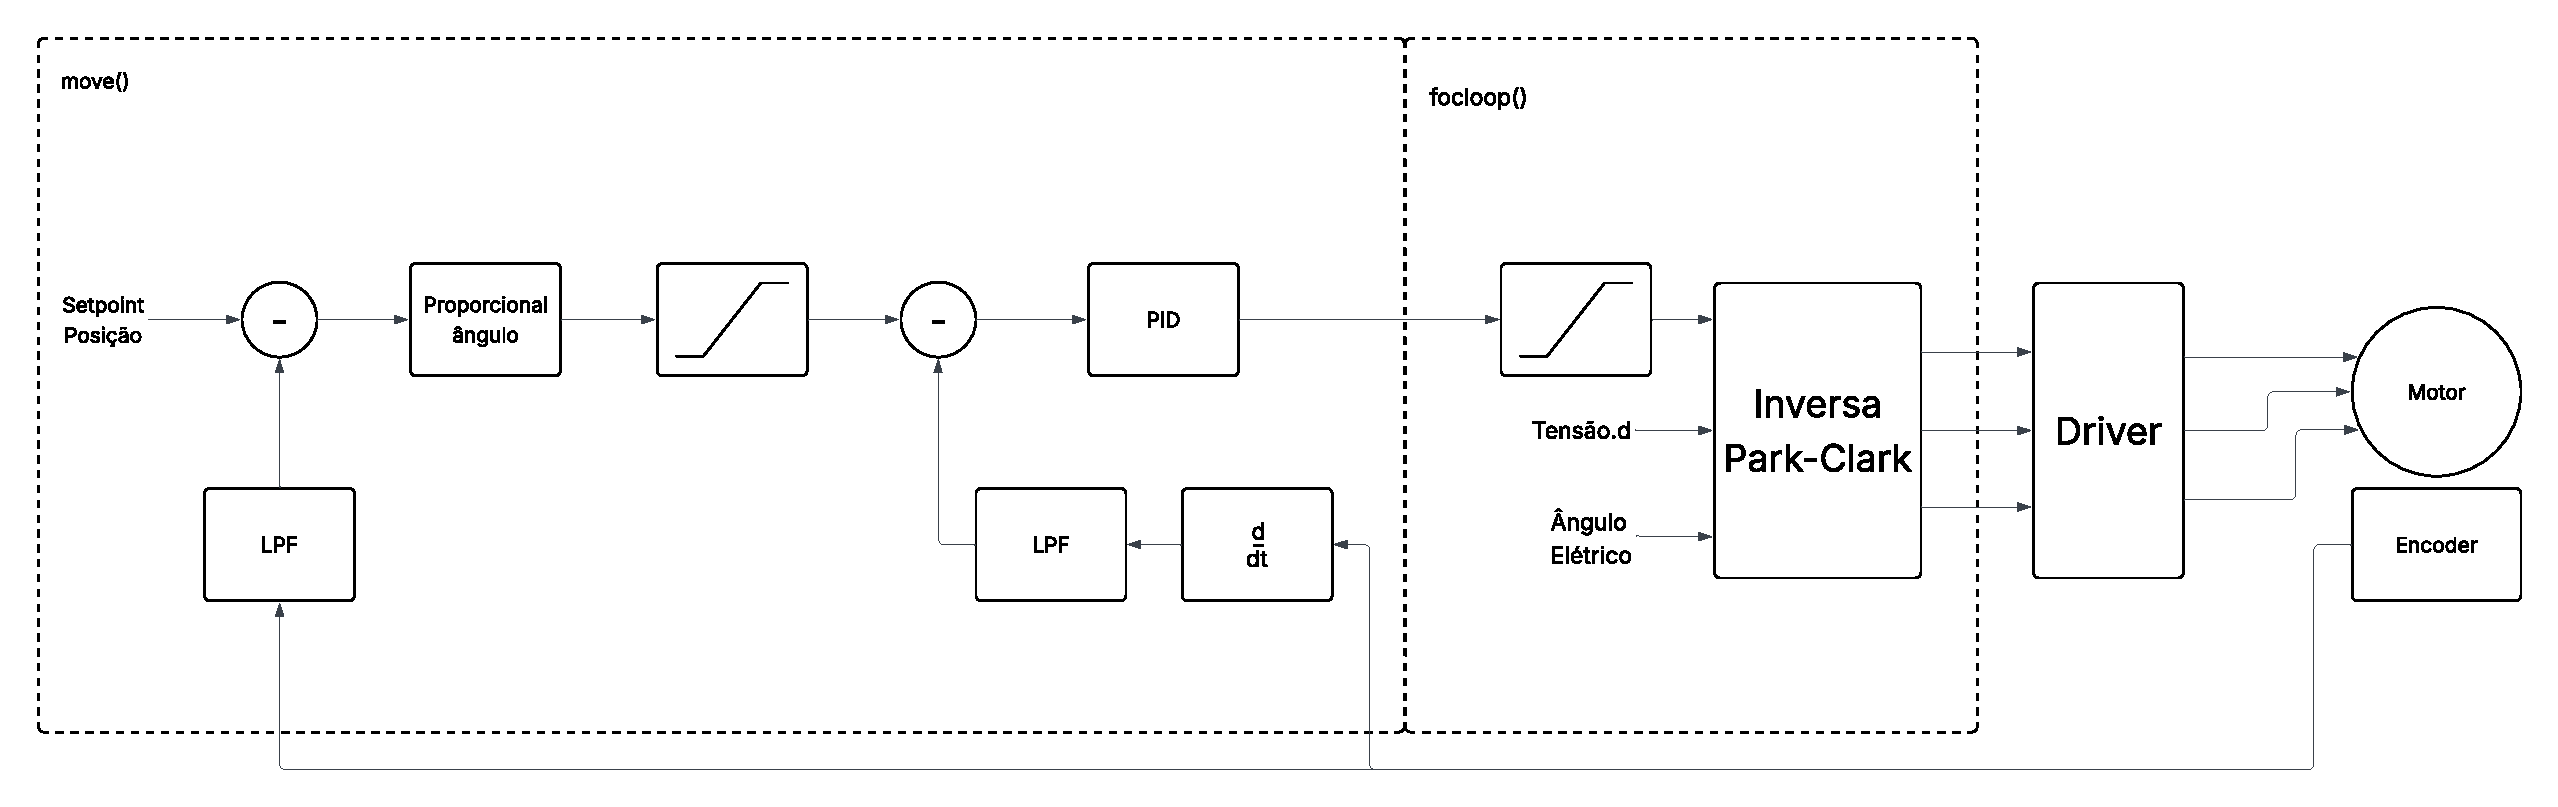
\includegraphics[width=\textwidth, keepaspectratio]{chapters/ch6_Controlo/assets/tese_controlo.pdf}
    \caption[Diagrama de Blocos do Algoritmo de Controlo em Cascata]{Diagrama de blocos do ciclo de controlo em cascata do algoritmo FOC via \emph{SimpleFOC}.}
    \label{fig:diagrama_malha_controlo}
\end{figure}

O ciclo de controlo em tempo real é instanciado no microcontrolador ESP32-S3 de forma determinística, sendo dividido em duas rotinas principais, a função \emph{move()} e a função \emph{focloop()}. 

A execução inicia-se na função \emph{move()}, responsável pelo controlo de posição de nível superior. Nesta rotina, o valor de referência (\emph{setpoint}) de posição angular é comparado com o sinal de realimentação de posição do \emph{encoder} magnético MT6835. Para mitigar o ruído de alta frequência inerente à leitura digital, este sinal de retorno atravessa previamente um filtro passa-baixas digital de primeira ordem, gerando o erro de posição angular do eixo. Este erro posicional é multiplicado por um ganho proporcional de ângulo, sendo o resultado tratado como a referência de velocidade angular para a malha interna. Antes de transitar para a etapa seguinte, o sinal passa por um bloco de saturação que restringe a velocidade dentro dos limites físicos de segurança do \emph{gimbal}. 

A velocidade de referência resultante é então comparada com a velocidade real do motor, calculada no instante de amostragem através da diferenciação numérica da posição do \emph{encoder} e filtrada por um segundo filtro passa-baixas. O erro de velocidade daí resultante é processado por um controlador PID de velocidade, cujo sinal de saída encerra a execução da função.

A variável de atuação gerada pelo PID de velocidade entra, subsequentemente, na rotina de controlo vetorial de baixo nível, a função \texttt{loopFOC()}. Inicialmente, o sinal passa por um limitador para respeitar as especificações elétricas e de tensão da bateria, sendo convertido na tensão de referência do eixo de quadratura ($V_q$), a qual está diretamente relacionada com o binário mecânico do motor.

O bloco matemático da transformada inversa de \emph{Park} e de \emph{Clarke} recebe a tensão $V_q$, a tensão no eixo direto ($V_d$) e o ângulo elétrico ($\theta_e$) e transformam em sinais direcionados às fases $A$, $B$ e $C$ do estator. Por fim, os sinais de comando digital atuam o \emph{driver} de potência (ponte inversora trifásica), completando o ciclo de controlo em tempo real.

%----------------------------------------------------------------------------------------

\section{Modelação e Identificação Experimental em Frequência}
\label{subsec:identificacao_frequencia}

Para projetar os controladores PID de forma analítica e garantir o cumprimento dos requisitos de estabilidade e seguimento, torna-se imperativo conhecer o modelo matemático que rege a dinâmica física de cada eixo do \emph{gimbal}. Para tal, optou-se por uma abordagem de modelação experimental baseada na resposta em frequência do sistema.

O método de identidade consistiu na realização de um varrimento de frequências. Utilizando o controlo de tensão da biblioteca \emph{SimpleFOC}, injetou-se um sinal de excitação sinusoidal contínuo na entrada de tensão de quadratura ($V_q$), com uma amplitude controlada, varrendo um espetro desde frequências baixas até ao limite da largura de banda do atuador. Em cada patamar de frequência, a resposta do motor foi monitorizada em tempo real através do \emph{encoder} magnético MT6835.

A partir da relação entre o sinal de excitação (entrada) e a resposta dinâmica do sistema (saída), procedeu-se ao levantamento do Diagrama de Bode. A análise gráfica deste comportamento experimental permitiu aproximar a dinâmica do eixo a uma Função de Transferência, $G(s)$, definida genericamente no domínio de Laplace pela Equação~\ref{eq:funcao_transferencia}:

\begin{equation}
    G(s) = \frac{\Theta(s)}{V_q(s)} = \frac{K}{s(\tau s + 1)} = \frac{K}{s^2\tau + s}
    \label{eq:funcao_transferencia}
\end{equation}

Onde $K$ representa o ganho estático do sistema e $\tau$ corresponde à constante de tempo mecânica. A presença do integrador puro na Equação~\ref{eq:funcao_transferencia} reflete a integração da posição de forma naturar por estár a atuar na tensão que é diretamente proporcional à velocidade.

De forma a caracterizar individualmente a resposta dinâmica de cada canal de atuação do \emph{gimbal}, o procedimento de varrimento de frequências foi executado de forma independente para o eixo de elevação (\emph{pitch}) e para o eixo de azimute (\emph{yaw}). Os diagramas de Bode obtidos experimentalmente encontram-se representados na Figura~\ref{fig:bode_identificacao_eixos}.

\begin{figure}[H]
    \centering
    % Subfigura Esquerda - Pitch
    \begin{subfigure}[b]{0.48\textwidth}
        \centering
        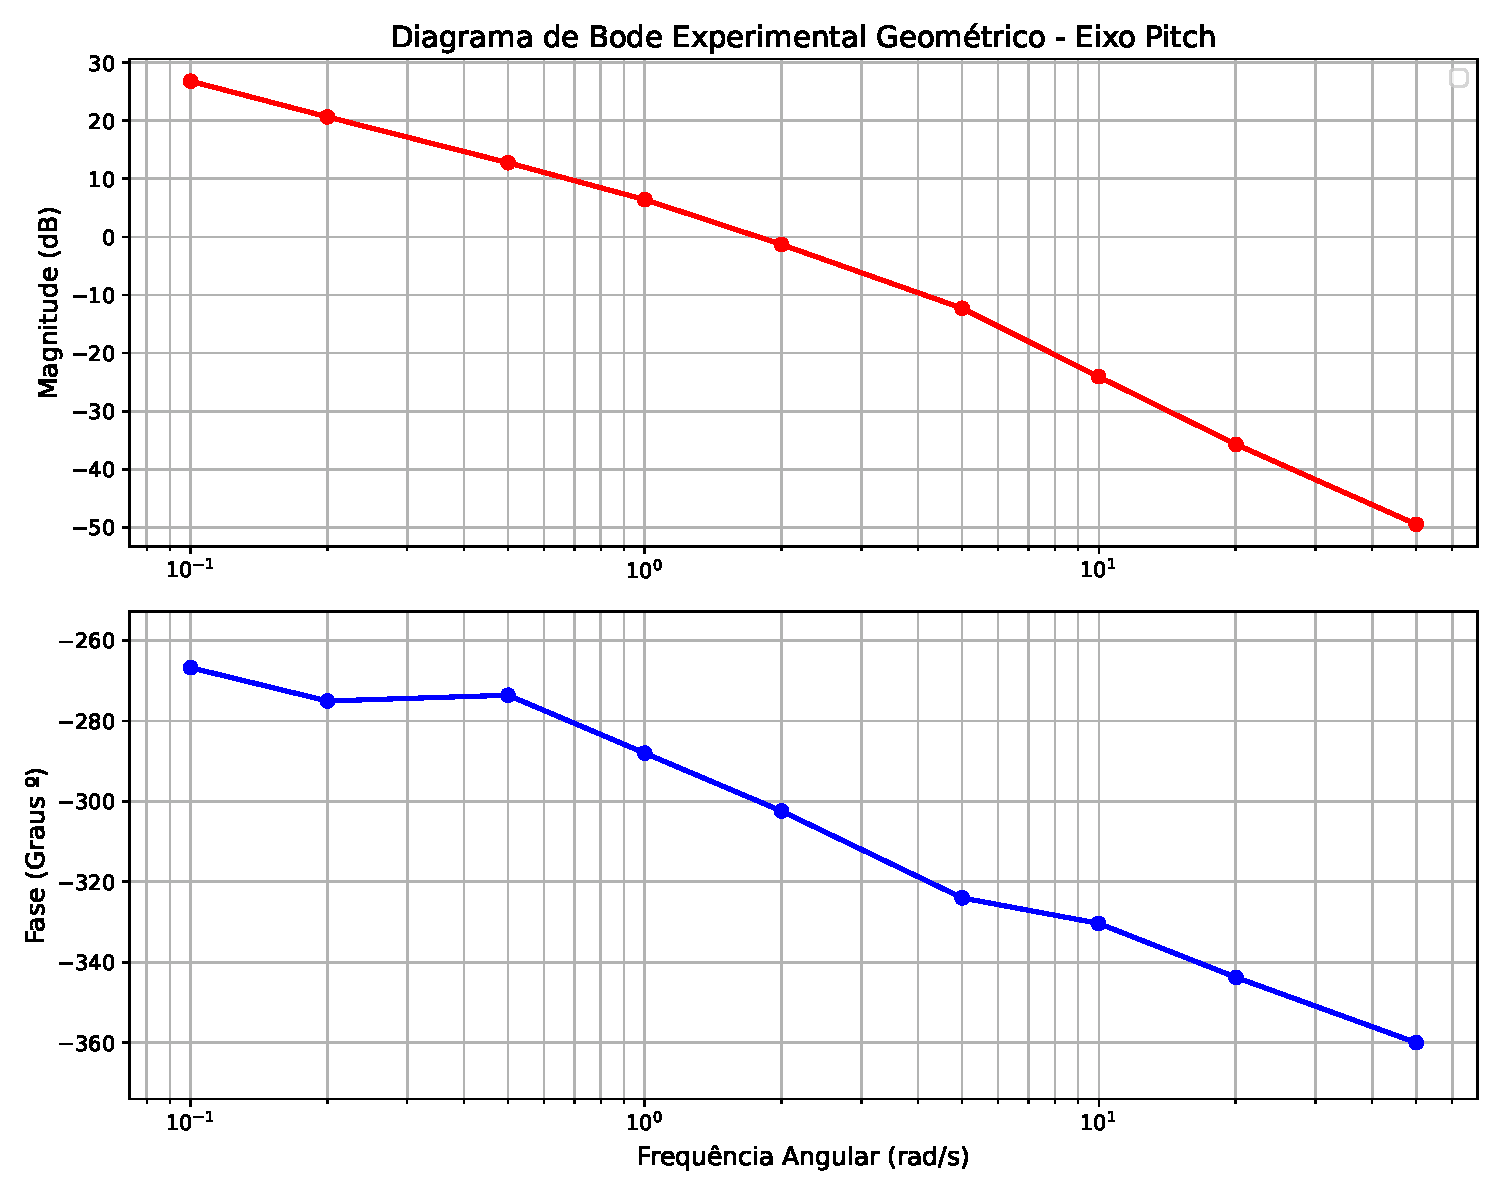
\includegraphics[width=\textwidth,keepaspectratio]{chapters/ch6_Controlo/assets/diagrama_bode_pitch.pdf}
        \caption{Eixo de \emph{Pitch}.}
        \label{fig:sub_bode_pitch}
    \end{subfigure}\hfill
    % Subfigura Direita - Yaw
    \begin{subfigure}[b]{0.48\textwidth}
        \centering
        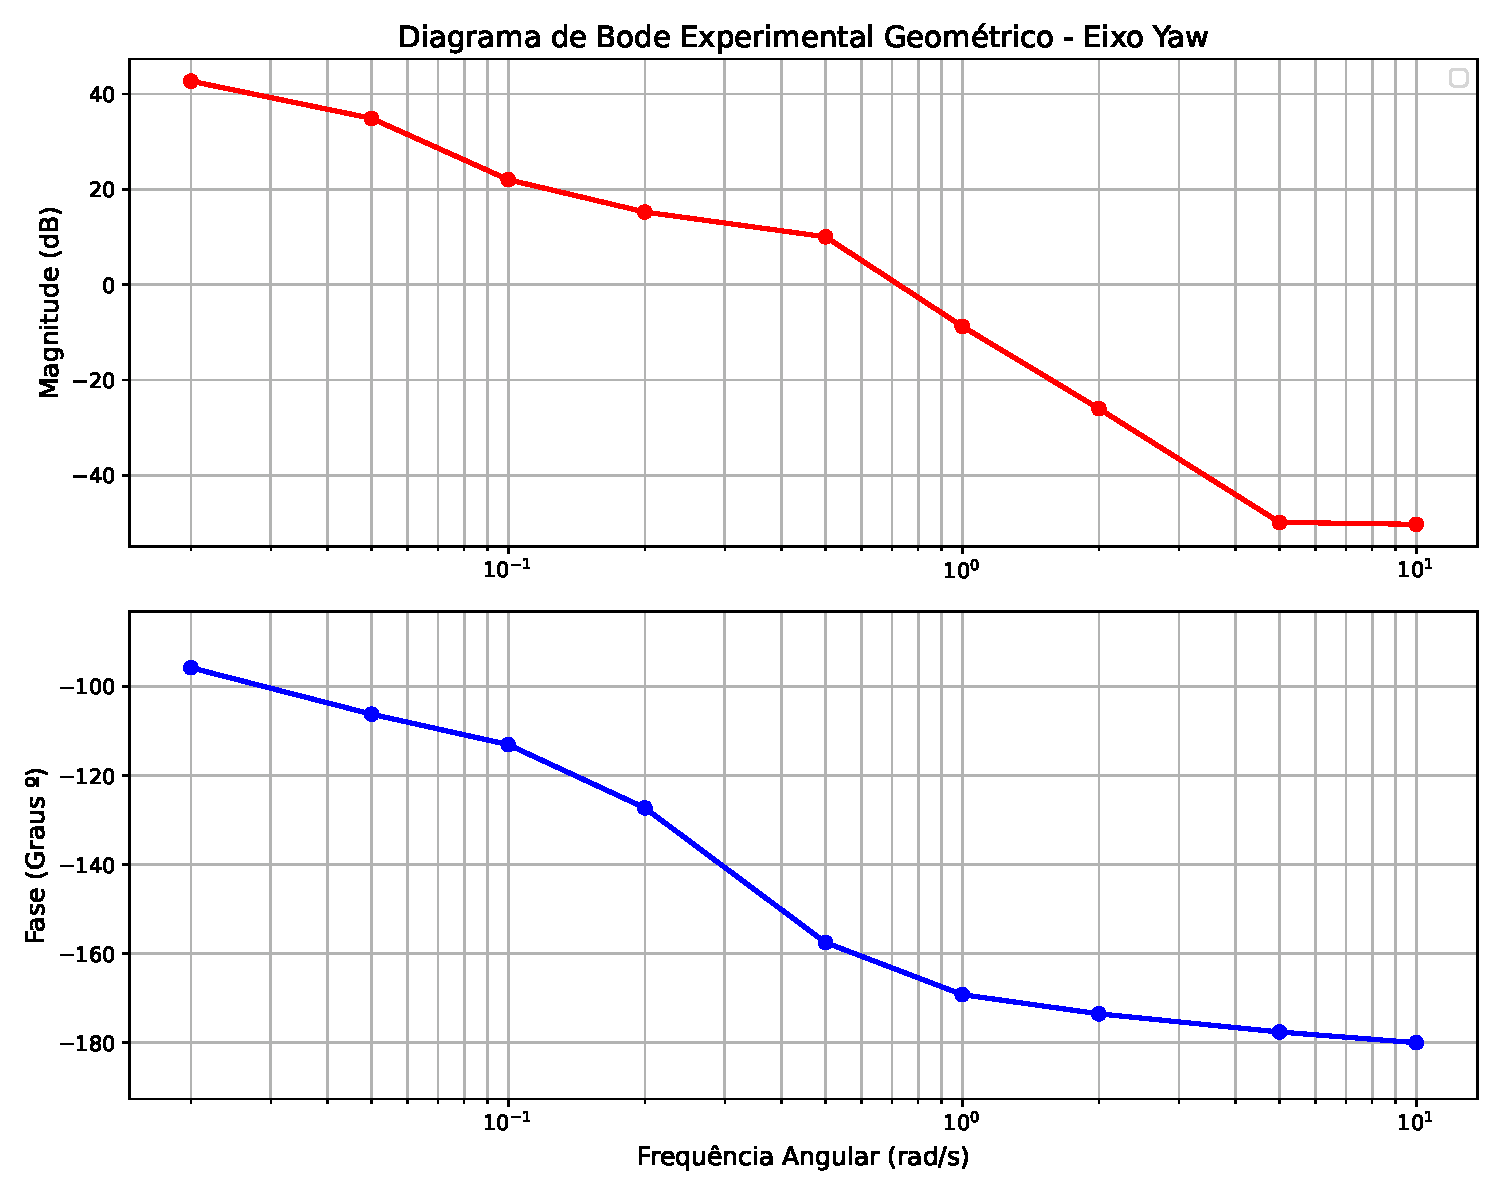
\includegraphics[width=\textwidth,keepaspectratio]{chapters/ch6_Controlo/assets/diagrama_bode_yaw.pdf}
        \caption{Eixo de \emph{Yaw}.}
        \label{fig:sub_bode_yaw}
    \end{subfigure}
    \caption[Diagramas de Bode Experimentais por Eixo]{Diagramas de Bode experimentais.}
    \label{fig:bode_identificacao_eixos}
\end{figure}

A nível de frequutilizou-se 50 rad/s e 10 rad/s como frequência máxima de pitch e yaw, respetivamente, dado que a frequências maiores não é possível detetar com certeza a fase e o ruído do sensor. A frequência minima foi selecionada para obter pelo menos uma decada antes do polo por forma a obter a fase em cerca de 90º. 

Os diagrama de bode obtido demonstra que ambos os motores apresentam uma fase de cerca de 90º graus em baixas frequencias dado polo presente na origem dado que o controlo em tensão é proporcional ao torque e que neste caso é diretamente convertido em velocidade.
\textbf{falar sobre os resultados referindo que começão a 90/270 dado ter um polo na origem e um polo mecânico (n sei se abordo o polo elétrico que é dificil medir)}

\textbf{abordar a função de transferencia retirada de cada diagrama de bode}


\section{Controlador de Seguimento}

Com as funções de transferência identificadas através do ensaio em frequência, constata-se que a tensão de quadratura $V_q(s)$ é diretamente proporcional ao binário eletromecânico aplicado às fases estatóricas, e a posição angular final de $\Theta(s)$ se caracteriza como um sistema de Tipo 1, devido à presença do integrador puro intrínseco. De modo a capacitar o \emph{gimbal} para o seguimento rigoroso do \ac{UAV} a uma velocidade constante limite sem erros posicionais, caracterizando-se por seguimento em rampa, projetou-se uma arquitetura de controlo baseada num compensador Proporcional-Integral com Ação Derivativa na Realimentação(PI-D). Nesta topologia, a ação derivativa foi aplicada exclusivamente ao sinal de realimentação de velocidade e não ao sinal de erro posicional, uma estratégia que visa eliminar por completo o fenómeno de \emph{setpoint kick}, que consiste em picos abruptos e saturações violentas na variável de atuação sempre que a referência de trajetória sofre alterações súbitas ou degraus gerados pelo algoritmo de visão computacional. Para reduzir o ruído produzido na velocidade procedeu-se à integração de um filtro passa-baixas digital de primeira ordem diretamente acoplado ao bloco derivativo, atenuando a amplificação do ruído de alta frequência decorrente da diferenciação numérica do sinal do \emph{encoder} magnético, garantindo que apenas as variações dinâmicas reais da velocidade influenciem a ação de controlo. Apoiado no modelo paramétrico linearizado da planta obtido previamente via Diagrama de Bode, desenvolveu-se um modelo de simulação computacional em ambiente \emph{Simulink}, a aproximar o ambiente virtual à realidade física do protótipo, operando à discretização temporal com o delta t igual ao verificado no controle físico, integraram-se não-linearidades estritas no modelo de simulação, designadamente os limites de saturação de tensão impostos pela eletrónica de potência dos \emph{drivers} e a zona morta (\emph{dead-band}) induzida pelo atrito estático presente nos rolamentos e nos pontos de contacto da estrutura fabricada em manufatura aditiva. A sintonia final e a otimização dos ganhos do controlador foram executadas recorrendo à ferramenta \emph{PID Tuner} do \emph{MATLAB}, através da qual se testaram iterativamente múltiplos perfis de compensadores com filtro na derivada para a malha. O objetivo deste processo de otimização consistiu em encontrar um equilíbrio de desempenho que maximizasse a largura de banda e garantisse uma resposta transiente extremamente rápida face à dinâmica de fuga da ameaça, assegurando, em simultâneo, que a ação de comando calculada não forçasse a saturação contínua da tensão do motor, prevenindo fenómenos de instabilidade.



%\begin{equation}
%    G_{pitch}(s) = \frac{\Theta_{pitch}(s)}{V_q(s)} = \frac{K}{s^2 + \frac{1}{\tau}s} =\frac{0.0}{s^2 + 0.0s}
%    \label{eq:tf_pitch}
%\end{equation}

%----------------------------------------------------------------------------------------

\section{Ensaios Experimentais do Controlador}
\label{sec:ensaios_pid}

%Com base nas funções de transferência experimentais obtidas na secção anterior, procedeu-se ao cálculo analítico dos parâmetros do controlador PID em cascata para ambos os eixos (\emph{pitch} e \emph{yaw}). Esta secção detalha a validação prática do comportamento dinâmico do sistema em bancada de ensaios.

\subsection{Resposta ao Degrau (Step Response)}
\label{subsec:resposta_degrau}
% Aqui deves descrever o ensaio de resposta a uma mudança abrupta de posição.
% Analisa graficamente os parâmetros: Overshoot (sobre-sinal), Rise Time (tempo de subida) e Settling Time (tempo de estabelecimento).

\subsection{Seguimento de Trajetória Dinâmica (Onda Triangular)}
\label{subsec:onda_triangular}
% Aqui deves descrever o ensaio com a onda triangular.
% Explica que a onda triangular mimetiza um alvo a mover-se com velocidade angular constante (entrada em rampa)
% e demonstra como o controlador lida com o erro em rampa e com as inversões abruptas de sentido de rotação.

\subsection{Resolução Máxima Experimental}
\label{subsec:resolucao_maxima}
\textbf{Posso deixar aqui? ou não faz sentido abordar o ensaio da resolução aqui?}
% Aqui deves apresentar os resultados do teste limite de resolução.
% Qual foi o menor degrau angular (em frações de grau ou radianos) que o gimbal conseguiu detetar, processar e corrigir de forma estável, validando o uso do encoder de 21 bits.

\begin{figure}[H]
\centering
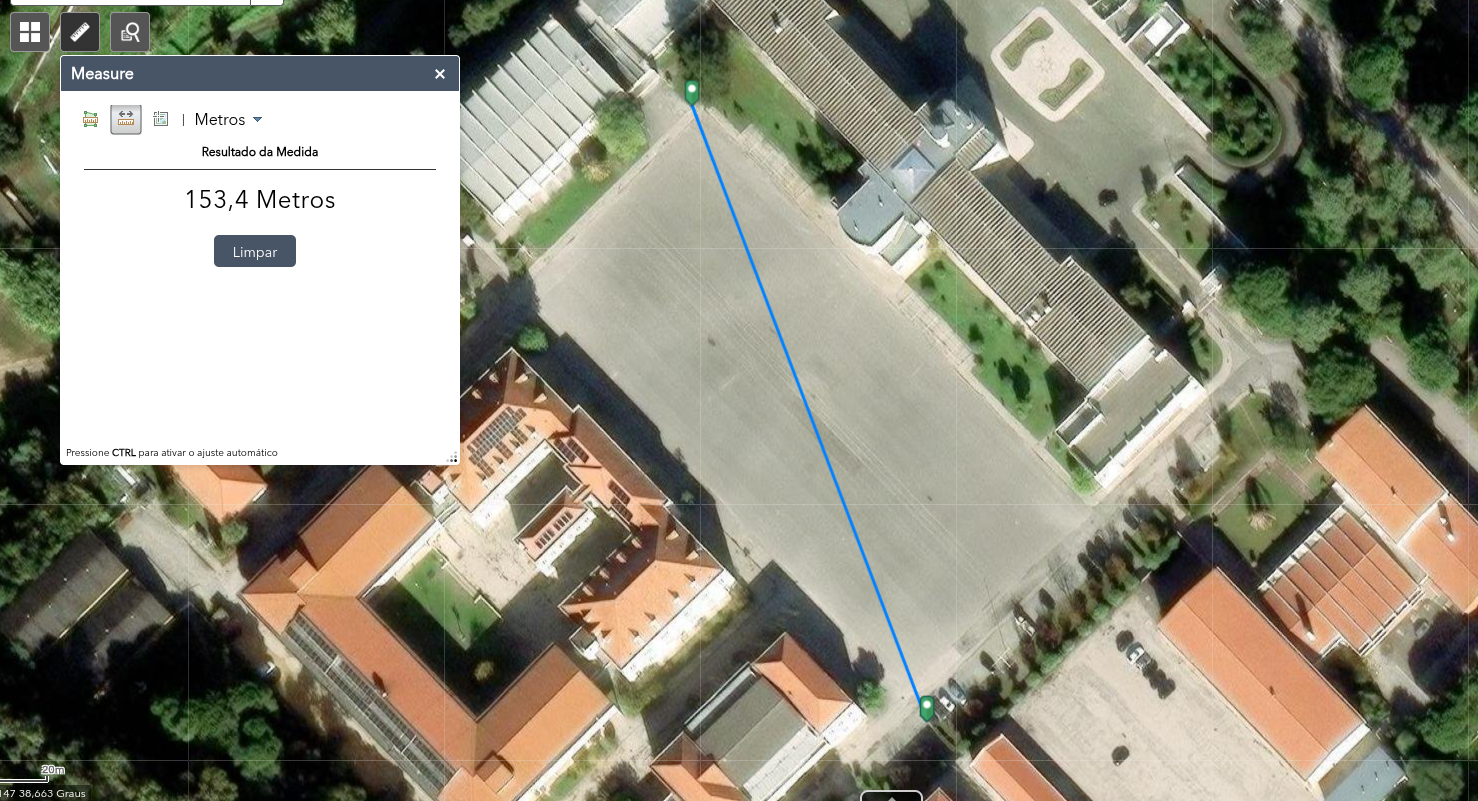
\includegraphics[width = 0.5\textwidth, keepaspectratio]{chapters/ch6_Controlo/assets/distancia_ensaio_laser.png}
\caption[A]{An }
\label{fig:dis}
\end{figure}
